%%%%%%%%%%%%%%%%%%%%%%%%%%%%%%%%%%%%%%%%%%%%%%%%%%%%%%%%%%%%%%%%%%%%%
%                       DESCRIPCIÓN GENERAL
%%%%%%%%%%%%%%%%%%%%%%%%%%%%%%%%%%%%%%%%%%%%%%%%%%%%%%%%%%%%%%%%%%%%%
\chapter{Descripción general del sistema}
En este capítulo se van a describir las características principales de la aplicación, las herramientas utilizadas para su desarrollo y los requisitos necesarios para poder llevar a cabo las funcionalidades descritas en la sección \ref{sec:1.2}.

\section{Presentación}
El objetivo principal de este trabajo fin de grado es la creación de una aplicación web que sea capaz de analizar un conjunto de páginas de \textit{Facebook} de manera automática. 

La figura (\ref{fig:general}) muestra un esquema general de la aplicación:

\begin{figure}[H]
\centering
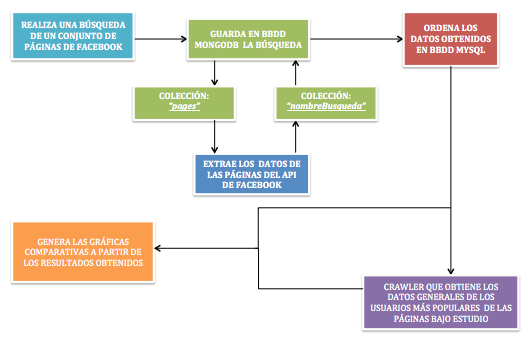
\includegraphics[width=5in]{figuras/esquemaGeneral.png}
\caption{Esquema general del proyecto} \label{fig:general}
\end{figure}

Siguiendo este esquema, primero el usuario debe indicar el nombre del estudio que va a realizar, el nombre de las páginas y el periodo de tiempo que lo engloban, y una dirección de correo electrónico para enviarle una notificación cuando la recopilación de datos haya finalizado. También debe seleccionar si desea que el estudio se haga sólo de las páginas de \textit{Facebook} o también de los usuarios más comunes. Una vez realizada la petición por parte del usuario, la aplicación web internamente se encarga de la recopilación de datos.
 
Para la recolección de los datos, primero guarda la búsqueda del usuario en una base de datos en MongoDB, en una colección llamada "pages". 

Acto seguido, realiza una petición al API de \textit{Facebook}, solicitando los datos contenidos en la sección \textit{Post to Page} de cada una de las páginas dentro del periodo de tiempo solicitado por el usuario. Esta petición devuelve los datos que son automáticamente guardados en la base de datos de MongoDB, en una colección creada con el mismo nombre que ha indicado el usuario para su estudio. 

A continuación, se procesan los datos en una base de datos relacional, MySQL, que permite estructurar los datos obtenidos de la Plataforma de \textit{Facebook}, guardando sólo aquellos campos que nos interesan y ordenándolos para facilitar su posterior procesado.

Una vez finalizado este paso, si el usuario ha seleccionado la opción del estudio de usuarios, por un lado se procede a la extracción de sus datos y por otro lado, se manda un primer informe al usuario de la aplicación con las gráficas de los datos obtenidos de \textit{Facebook}. Proceso que se repite cuando la recopilación de datos de los usuarios haya finalizado.    

Se trata de una aplicación clara y sencilla en la que los usuarios puedan comparar el análisis de diferentes páginas de \textit{Facebook} dentro de su sesión, llevando un historial que almacena todas las peticiones realizadas. 

\section{Requisitos necesarios}
En esta sección se van a definir los requisitos necesarios para el desarrollo técnico de la aplicación propuesta. También se definen los requisitos y restricciones de las tecnologías utilizadas.
\subsection{Requisitos de la aplicación}
A continuación se enumeran todos los requisitos y necesidades que se considera que debe realizar la herramienta a desarrollar, que afectan sólo al portal web. 
\begin{enumerate} \itemsep4pt \parskip0pt
\item \textbf{Accesible desde distintos navegadores}

Los navegadores más comunes, "Mozilla Firefox", "Google Chrome", "Safari", "Internet Explorer", podrán utilizar la aplicación.
\item \textbf{Idioma} \\
El idioma de la aplicación será el español.
\item \textbf{Registro de usuarios} \\
El usuario deberá registrarse previamente para usar la  aplicación.
\item \textbf{Inicio de sesión} \\ 
El usuario deberá haber iniciado sesión con una cuenta registrada para acceder a la aplicación.
\item \textbf{Nueva búsqueda: Nombre estudio} \\
El usuario deberá indicar el nombre del estudio que quiere realizar.
\item \textbf{Nueva búsqueda: Nombre páginas de Facebook} \\
El usuario deberá indicar el nombre de las páginas que quiere analizar, asegurándose primero de que estas páginas contengan la sección \textit{Post to Page}.
\item \textbf{Nueva búsqueda: Periodo del estudio} \\
El usuario deberá indicar la fecha de inicio del estudio, es decir, desde cuando quiere que sea el primer comentario recogido en el estudio hasta la fecha actual. 
\item \textbf{Nueva búsqueda: Correo Electrónico} \\
El usuario deberá indicar una cuenta de correo electrónico donde se le enviará una notificación cuando la recopilación de datos haya acabado. 
\item \textbf{Nueva búsqueda: Opción informe de las páginas}\\
Si el usuario selecciona esta opción se procederá a la recolección de datos de las páginas indicadas obteniéndolos del API de \textit{Facebook}, y se representarán las gráficas comparativas con los resultados obtenidos.
\item \textbf{Nueva búsqueda: Opción informe de los usuarios} \\
Si el usuario selecciona esta opción se procederá a la extracción de datos de los usuarios que más comentan en dicha sección de \textit{Facebook}. Se obtendrán los datos de los usuarios de su fecha y lugar de nacimiento, edad y ocupación profesional mediante un \textit{crawler}.
\item \textbf{Historial de búsquedas} \\
Los usuarios tendrán acceso a todas las búsquedas que hayan realizado en la aplicación, se mostrarán en una tabla.
\item \textbf{Ver análisis} \\
Los usuarios dentro del historial de búsqueda podrán acceder a ver el análisis de cada uno de los estudios, se representarán las gráficas más representativas de los datos obtenidos. 
\item \textbf{Cerrar sesión} \\
Los usuarios podrán cerrar sesión cuando quieran, para mantener seguros sus estudios. 
\item \textbf{Web responsiva} \\
La interfaz web deberá adaptarse a cualquier tamaño de pantalla.
\item \textbf{Lenguajes de programación} \\
Los lenguajes de programación para el desarrollo de la aplicación serán: Java, JSP, HTML, CSS, XML, JavaScript y jQuery.
\end{enumerate}

\subsection{Requisitos de Facebook}
En este epígrafe se describirán los requisitos que Facebook impone para el correcto desarrollo de la aplicación que se pretende seguir. 
\begin{enumerate} \itemsep4pt \parskip0pt
\item \textbf{Soporte HTTP}\\
El servidor donde se aloje debe soportar peticiones HTTP Get y Post.
\item \textbf{Cuenta en Facebook} \\
Para poder acceder a \textit{Facebook}, se debe tener creada una cuenta en dicha red social.
\item \textbf{Cuenta de desarrollador} \\
Para poder acceder a la Plataforma de \textit{Facebook} y a su API, se debe crear crear una cuenta de desarrollador, esto es, aceptar los permisos y condiciones que indican desde una cuenta de \textit{Facebook} de usuario.
\item \textbf{Crear una aplicación en Facebook}\\
Para poder hacer peticiones a la API se necesita crear una aplicación dentro de la Plataforma, que proporcionará las credenciales necesarias para dichas peticiones.
\end{enumerate}

\subsection{Requisitos del crawler}
En este apartado se definirán las condiciones necesarias para poder ejecutar el \textit{crawler} en el entorno adecuado.
\begin{enumerate} \itemsep4pt \parskip0pt
\item \textbf{Máquinas virtuales con interfaz gráfica}\\
Para poder simular la acción de un usuario normal de \textit{Facebook} que recopile los datos de los usuarios a los que visita, se necesitará acceso a máquinas virtuales con entorno gráfico, donde se ejecutará el \textit{crawler} que lanzará instancias de un navegador para simular esta acción.
\item \textbf{Java} \\
El lenguaje de programación será Java, por lo que habrá que instalar el entorno de Java en la máquinas que se vaya a ejecutar. 
\item  \textbf{Número de identificación de los usuarios de \textit{Facebook}} \\
Se necesitarán los \textit{ids} de aquellos usuarios que se vayan a analizar mediante el \textit{crawler}.
\item  \textbf{Distribución del crawler} \\
Se utilizará un software de distribución de paquetes, RabbitMQ, para optimizar el tiempo de ejecución del \textit{crawler}. Desde la aplicación se mandará a cada máquina virtual, mediante este mecanismo, el trabajo que debe realizar cada una.
\end{enumerate}

\subsection{Requisitos de desarrollo}
Por último se expondrán los requisitos necesarios para la elaboración de este proyecto.
\begin{enumerate} \itemsep4pt \parskip0pt
\item \textbf{Espacio para el trabajo} \\
Se dispondrá de una espacio lo suficientemente amplio para poder albergar el equipo de trabajo.
\item \textbf{Ordenador} \\
Se necesitará un ordenador para el desarrollo del trabajo fin de grado.
\item \textbf{Conexión a internet} \\
Se necesitará conexión a Internet para la completa realización del proyecto.
\item \textbf{Servidor} \\
Se necesitará un servidor donde alojar las máquinas virtuales.
\item \textbf{Servidor web y bases de datos}
Se requerirá un servidor web donde alojar la aplicación web y deberá soportar el almacenamiento de los datos en bases de datos. 
\end{enumerate}

\section{Alternativas de implementación del sistema}
\subsection{Alternativas del lenguaje}
Una vez planteadas las tecnologías a desarrollar y los requisitos necesarios, se tuvieron en cuenta las posibilidades de los lenguajes de programación para aplicar al proyecto. 
Para el desarrollo de una aplicación web se utilizan tres lenguajes indispensables, HTML, CSS y JavaScript, para el diseño de las vistas. Sin embargo, para integrar la aplicación con la API de \textit{Facebook} y para el manejo de las bases de datos se pueden utilizar varios lenguajes como Java, Python o Ruby, que disponen de librerías para facilitar el acceso a estas tecnologías.
También se analizaron las posibilidades para el desarrollo del "\textit{crawler}" basado en la herramienta de pruebas de Selenium-WebDriver. Esta herramienta está completamente implementada y soportada en Java, Ruby, Python y C\#. 
\subsection{Evaluación de las alternativas de lenguaje y elección de la solución}
Como las alternativas disponibles para el desarrollo de las tecnologías que conforman el núcleo de este trabajo fin de grado se podían desarrollar indistintamente en varios lenguajes, finalmente se decidió el lenguaje de programación Java. 
Una de las ventajas de decidir Java es que es programación orientada a objetos, simplifica mucho el código y el desarrollo definiendo los objetos necesarios y reutilizándolos. Otra de las ventajas es que es multiplataforma, funciona en todos los entornos disponibles. Es completamente gratis y no depende de ninguna licencia. 
\subsection{Alternativas de las bases de datos}
A la hora de decidir el tipo de bases de datos a utilizar, se tuvo que tener en cuenta el motor principal de este trabajo fin de grado, que es la API de Facebook. Las consultas que se realizan a Facebook, la API las devuelve en formato JSON, y con una estructura variable, dependiendo de los datos que proporciona cada página. 
Por este motivo, se estudió la posibilidad de usar una base de datos NoSQL, que permitiera almacenar los datos sin un esquema predefinido.
Existen varias posibilidades de bases de datos no relacionales como son Cassandra, Redis, MongoDB y CouchDB.
Pero por otro lado, de cara al análisis de datos que esta aplicación recogerá, se consideró que sería conveniente tener una base de datos organizada, almacenando los datos de interés para el análisis. Varias de las alternativas planteadas fueron: MySQL, Access, PostgreesSQL, Microsoft SQL.  
\subsection{Evaluación de las alternativas de bases de datos y elección de la solución}
Dentro de los tipos de bases de datos relacionales, se eligió una base de datos en MySQL, porque aunque todos los tipos cumplían los requisitos necesarios para la implementación de este trabajo fin de grado, MySQL se caracteriza por la rapidez de acceso a la información, punto interesante de cara a cargar los datos en una página web. Además el volumen de datos almacenado no será muy grande, otro aspecto por los que se eligió MySQL. 

En cuanto a las opciones de bases de datos no relacionales la elección fue más fácil. Se eligió MongoDB porque se pueden almacenar los datos BSON directamente, que es una evolución de JSON, esto facilita las peticiones realizadas a la API de Facebook, pudiendo almacenar el JSON que devuelve, sin tener que comprobar si están todos los campos, o si añade uno nuevo. Además de que es un bastante rápido a la hora de ejecutar las operaciones.
\subsection{Alternativas del diseño web}
El Frontend que conformará la interfaz de usuario, para esta parte se utilizará HTML, CSS para definir los estilos y JavaScript y jQuery para añadir efectos y funcionalidades a la página. 
Por otro lado, para el Backend, se estudiaron las distintas posibilidades para generar las páginas de forma dinámica. En esta parte, hubo que decidir el lenguaje de programación adecuado. Estos lenguajes, en el lado del servidor, buscarán la información en una base de datos para mostrarla en la interfaz. Existen varias posibilidades como son PHP, Python, Ruby, ASP.NET o Java.
\subsection{Evaluación de las alternativas de diseño web y elección de la solución} \label{sec:3.3.6}
El diseño web fue el último punto de este proyecto que se decidió, debido a que la importancia del trabajo era recopilar los datos de Facebook. Por tanto, una vez definido como lenguaje de programación Java, y teniendo tanto el \textit{crawler} como el programa que accede a la API de Facebook en Java, se estudiaron las opciones disponibles de hacer una aplicación que implementara sin ningún tipo de problema los scripts comentados. Por esta misma razón se decidió realizar la aplicación web en la plataforma Java, utilizando Spring, que es un framework para el desarrollo de aplicaciones para la plataforma Java. Concretamente. Spring-MVC, módulo que implementa la arquitectura de Modelo-Vista-Controlador.

Destacar que el diseño de la aplicación se ha llevado acabo utilizando dos plantillas de Bootstrap. Bootstrap es un \textit{framework} CSS, que permite dar forma a un sitio web utilizando librerías CSS ya definidas. Una de las plantillas se ha utilizado para los formularios de Inicio de Sesión y de Registro, esta plantilla se llama  "Sign In Bootstrap Template" y se puede encontrar en el enlace \cite{login}. Estas plantillas se han modificado acorde a la estética de la aplicación. La otra plantilla se ha utilizado para el formulario de una nueva búsqueda, y ha definido el estilo que sigue la aplicación, se llama "Multi Step Registration Form" y se puede encontrar en el enlace \cite{step}. 
\section{Entorno de desarrollo utilizado}

\subsection{Eclipse IDE for Java EE Developers}

El programa utilizado para implementar el código de la aplicación es Eclipse \cite{3}. Es un programa informático compuesto por un conjunto de herramientas de programación de código abierto multiplataforma. 

Para desarrollar este proyecto se han utilizado dos plugins disponibles en el entorno de desarrollo. Un plugin es un complemento que se instala en el entorno de desarrollo, facilitan y agilizan el desarrollo.

Un plugin utilizado es el de Maven \cite{3}, Maven es una herramienta de gestión de proyectos. Se basa en un fichero central pom.xml, donde se definen todas las dependencias necesarias para el proyecto. Maven maneja las dependencias del proyecto, se las descarga y las añade al \textit{classpath}. Otro puglin necesario es el de Spring, Spring es un \textit{framework} para el desarrollo de aplicaciones de código abierto para la plataforma Java. En este proyecto se ha utilizado la versión 3 del \textit{framework}, que permite definir una arquitectura de software Modelo-Vista-Controlador. Esta arquitectura define por un lado los componentes para la representación de la información, y por otro lado para la interacción del usuario.

En las figuras (\ref{fig:esqEclipseB}) y (\ref{fig:esqEclipseF}) se presenta el esquema seguido para el desarrollo del trabajo de fin de grado en Eclipse. 

\begin{figure}[H]
\centering
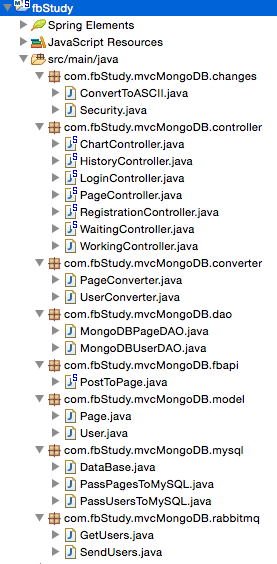
\includegraphics[width=3.2in]{figuras/esquemaBackend.png}
\caption{Esquema TFG en Eclipse. Parte 1} \label{fig:esqEclipseB}
\end{figure}

\begin{figure}[H]
\centering
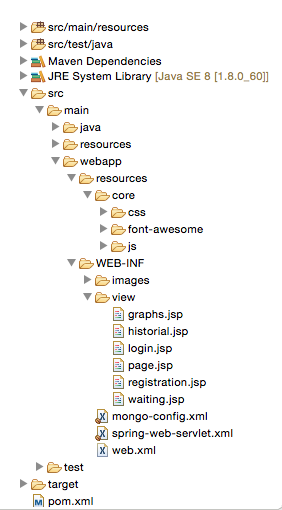
\includegraphics[width=3.5in]{figuras/esquemaFrontend.png}
\caption{Esquema TFG en Eclipse. Parte 2} \label{fig:esqEclipseF}
\end{figure}

Como se puede observar en los esquemas anteriormente mostrados, dentro de la carpeta "src/main/java" se ha definido un paquete para cada una de las funcionalidades implementadas, además de las propias necesarias para el correcto funcionamiento de la aplicaciones web siguiendo la estructura MVC. 

Por otro lado en la carpeta "webapp" se definen todas las vistas necesarias para la aplicación web, además de los estilos y plantillas utilizadas, y la configuración del servidor web, que se describe en el siguiente apartado \ref{sec:1.2}.

A continuación en las tablas (\ref{tab:clases1}) y (\ref{tab:clases2}), se detalla la funcionalidad de las clases mostradas en los esquemas anteriores:
\begin{table}[H]
	\centering
	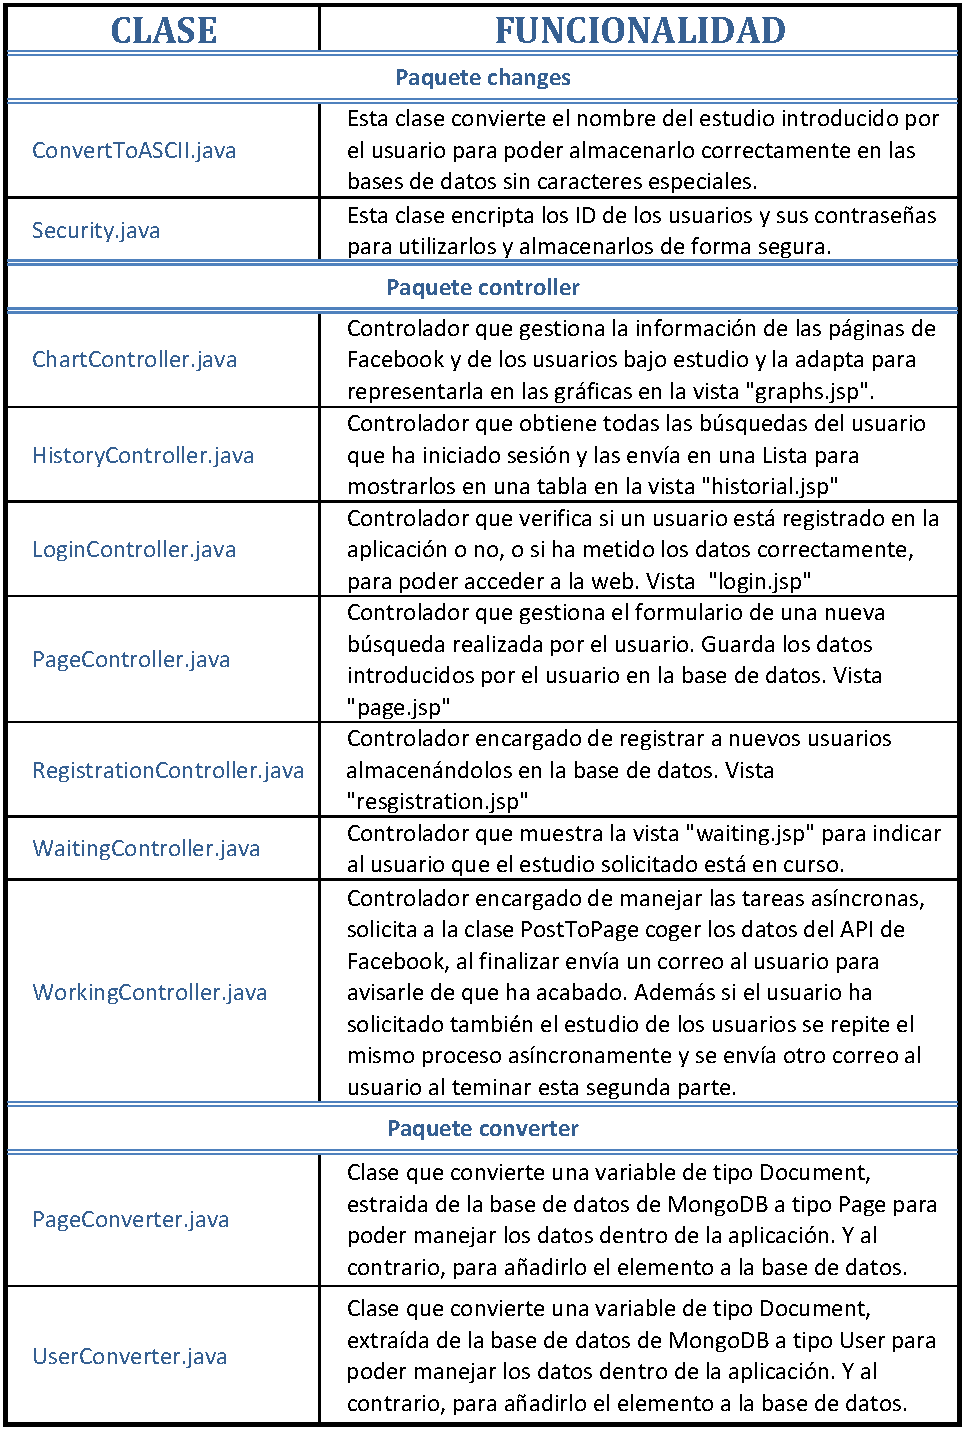
\includegraphics[width=5.2in]{PDF/Clasesjava1.pdf}
	\caption{Clases de java definidas en el proyecto. Parte 1}
	\label{tab:clases1}
\end{table}
\begin{table}[H]
	\centering
	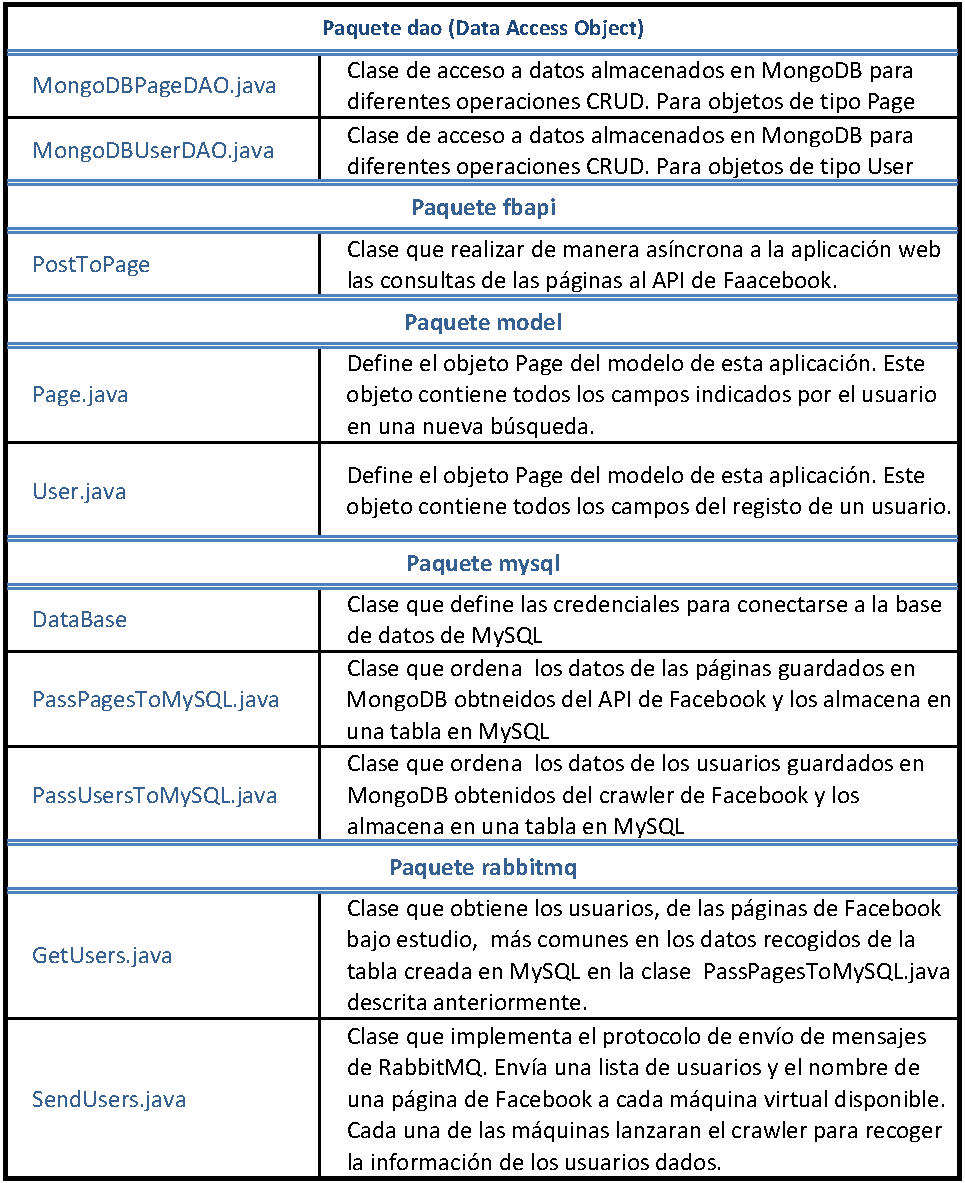
\includegraphics[width=5in]{PDF/Clasesjava2.pdf}
	\caption{Clases de java definidas en el proyecto. Parte 2}
	\label{tab:clases2}
\end{table}
\subsection{Servidor web Jetty} \label{sec:1.2}
\begin{figure}[H]
\centering

\includegraphics[width=2in]{figuras/logoJetty.jpg}
\caption{Logo Servidor Web Jetty} \label{fig:logoJetty}
\end{figure}

Jetty es un Servidor Web y Contenedor de \textit{Servlet}s preparado para ser embebido en las aplicaciones. Es un proyecto de software libre y está completamente basado en Java. 
Los motivos por los que se ha usado este servidor en concreto son los siguientes: \\
\begin{itemize} \itemsep4pt \parskip0pt
\item Es ligero y eficiente
\item Está alojado en Eclipse
\item Basado en Java
\item Soporta peticiones HTTP POST y GET
\item Procesa peticiones asíncronas, capaz de manejar el mecanismo de consulta larga
\end{itemize}

Además de cumplir todos los requisitos necesarios para este proyecto, otro de los motivos por los que se ha utilizado es por la simplicidad de su configuración, basta con definirlo en un fichero XML o en una clase java e incluir sus dependencias en el fichero pom.xml. Con estos dos pasos, la aplicación se ejecuta directamente desde este servidor web.

\begin{figure}[H]
\centering
{
\setlength{\fboxsep}{0pt}
\setlength{\fboxrule}{1pt}
\fbox{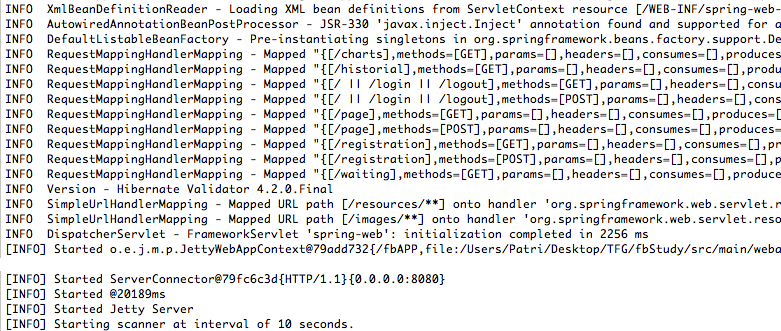
\includegraphics[width=6in]{figuras/ejemplolog.png}}
}
\caption{Registro del servidor web Jetty} \label{fig:log}
\end{figure}


%%%%%%%%%%%%%%%%%%%%%%%%%%%%%%%%%%%%%%%%%%%%%%%%%%%%%%%%%%%%%%%%%%%%%
%                       DESCRIPCIÓN DETALLADA
%%%%%%%%%%%%%%%%%%%%%%%%%%%%%%%%%%%%%%%%%%%%%%%%%%%%%%%%%%%%%%%%%%%%%
\chapter{Funcionamiento del sistema}

Para explicar en profundidad el funcionamiento de la aplicación web, se va a describir dividiéndolo en dos grandes grandes bloques, por un lado la parte del cliente, lo que el usuario ve, denominado frontend, y por otro lado la parte del servidor, cómo está distribuido el sistema para poder realizar todas las funcionalidades, denominado backend.

\section{Frontend}
En el frontend se define la interfaz de usuario. Como ya se ha descrito en la sección (\ref{sec:3.3.6}), la aplicación web está basada en Spring MVC. Se trata de un Modelo-Vista-Controlador. 

En esta sección se va a definir la Vista, que depende directamente del Modelo que se ha definido para que el usuario pueda interactuar con la aplicación. Además de indicar qué acciones realiza el Controlador para el correcto funcionamiento de cada una de las vistas detallas.

En el Modelo de esta aplicación se han diseñado dos objetos: 
\begin{itemize} \itemsep4pt \parskip0pt
\item Modelo User: define todos los campos de información relacionados con el usuario.  
\item Modelo Page: define todos los campos de información relacionados con la búsqueda de páginas.
\end{itemize}
Una vez definido el Modelo, la Vista ya puede interactuar con ellos mediante el Controlador que los maneja. 
Un Controlador responde a eventos, acciones del usuario, e invoca peticiones al Modelo cuando se hace alguna solicitud sobre la información. Cada Controlador se encarga de una vista, definidos en la tabla (\ref{tab:clases1}). 

Para facilitar el desenlace de este apartado en la figura (\ref{fig:web}) representa un diagrama del funcionamiento de la web básico.
\begin{figure}[H]
\centering
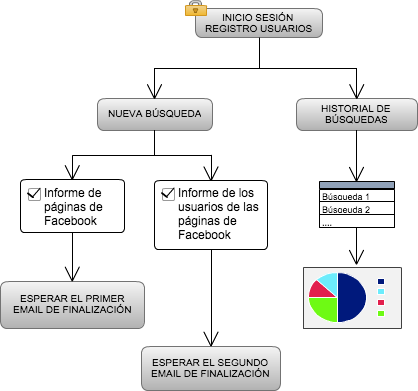
\includegraphics[width=3in]{figuras/appWeb.png}
\caption{Esquema funcionamiento frontend} \label{fig:web}
\end{figure}
Cada una de las pantallas está definida en una vista distinta que se definen a continuación por separado, explicando en detalle cada una de las acciones que el usuario puede realizar. 
\subsection{Registration}
\begin{figure}[H]
\centering
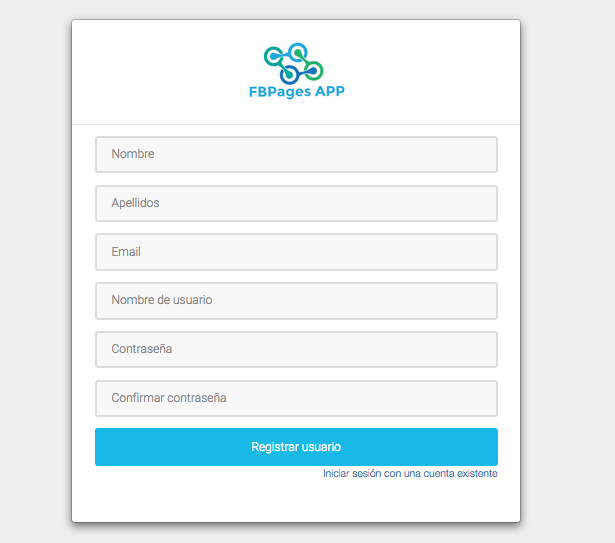
\includegraphics[width=4in]{figuras/registro.png}
\caption{Captura de pantalla del formulario de Registro} \label{fig:registration}
\end{figure}
En esta vista se define un formulario con un objeto de tipo "User", donde el usuario debe introducir todos los datos relacionados con su perfil, para poder crear una cuenta nueva en la aplicación. 

El controlador "RegistrationController.java" se encarga de comprobar que el usuario haya rellenado todos los campos del formulario, y que los datos introducidos sean correctos, en concreto que el campo email, se corresponda con una dirección de correo electrónico, y que la contraseña introducida coincida con la de verificación. 

Si el formulario es correcto, se crea un nuevo usuario que se almacena en la base de datos en la colección "users". 

\subsection{Login}

\begin{figure}[H]
\centering
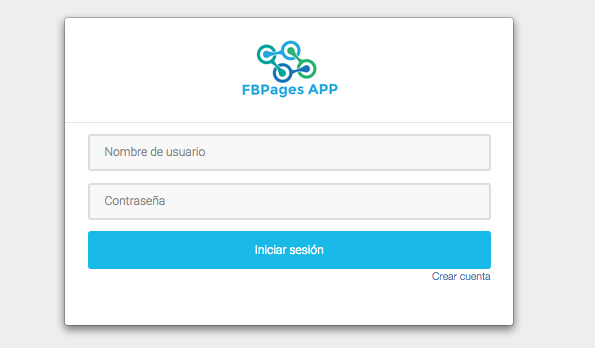
\includegraphics[width=5in]{figuras/login.png}
\caption{Captura de pantalla del formulario de Inicio de Sesión} \label{fig:login}
\end{figure}

En esta vista se presenta el formulario de inicio de sesión del usuario. Para poder acceder a la aplicación se requiere estar previamente registrado. 

De forma similar a la anterior vista, el controlador "LoginController.java" se encarga de que el usuario haya introducido bien el nombre de usuario y la contraseña, de ser así, se conecta con la base de datos y comprueba que exista dentro de la colección "users". Si existe, le da acceso a la aplicación, y si no le indica que no existe el usuario.
\subsection{Búsqueda} \label{sec:4.1.3}

Esta es la pantalla principal de la aplicación, aquí el usuario definirá las características del estudio que quiere realizar. 
Este formulario se define mediante el modelo "Page". Para facilitar la búsqueda al usuario, el formulario se ha dividido en cuatro pasos. Cada paso, está formado por un formulario sencillo, incluyen una breve explicación de los datos que se deben introducir.

A continuación se explica cada uno de los pasos brevemente, los campos necesarios en cada uno y además se muestra su aspecto visual: \\
\\
\begin{itemize} \itemsep4pt \parskip0pt
\item Paso 1/4 \\
\begin{figure}[H]
\centering
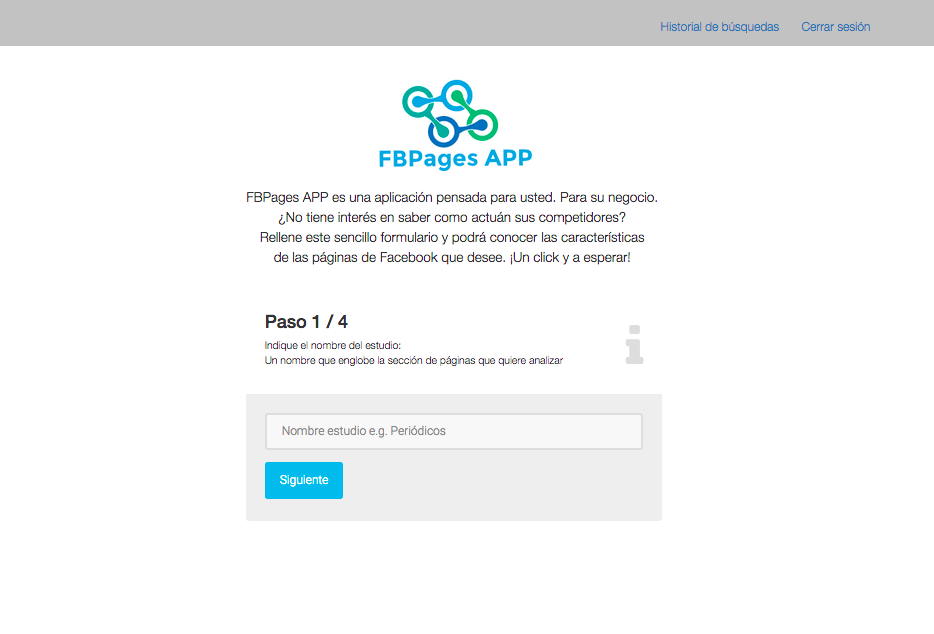
\includegraphics[width=4.5in]{figuras/paso1.png}
\caption{Captura de pantalla del Paso 1} \label{fig:paso1}
\end{figure}
El usuario debe indicar el nombre del estudio que va a realizar
\item Paso 2/4 \\
\begin{figure}[H]
\centering
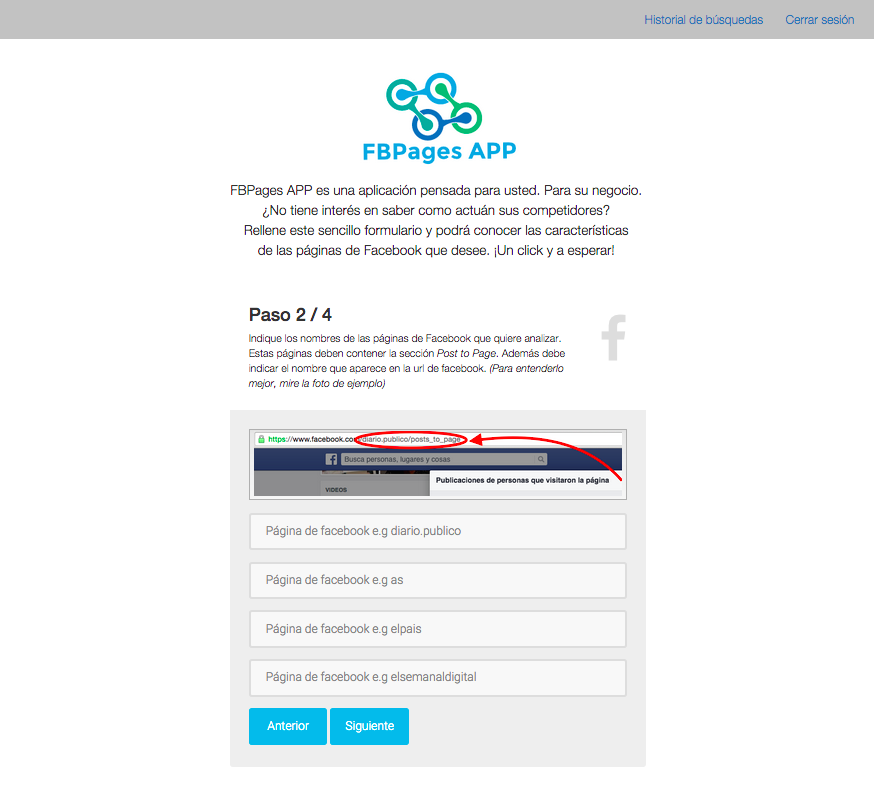
\includegraphics[width=4.5in]{figuras/paso2.png}
\caption{Captura de pantalla del Paso 2} \label{fig:paso2}
\end{figure}
El usuario debe introducir el nombre de las cuatro páginas de Facebook que quiere analizar. Como se puede observar en la figura (\ref{fig:paso2}), se ha introducido una imagen explicativa de la comprobación que debe hacer el usuario antes de añadir una página al formulario, para saber si dicha página contiene la sección \textit{Post To Page}, explicada anteriormente en el presente documento. Si contiene dicha sección, el nombre que debe introducir el usuario en el formulario, es el que aparece en la url de Facebook, para asegurarse de que es la página correcta la que se va a analizar. 
\begin{figure}[H]
\centering
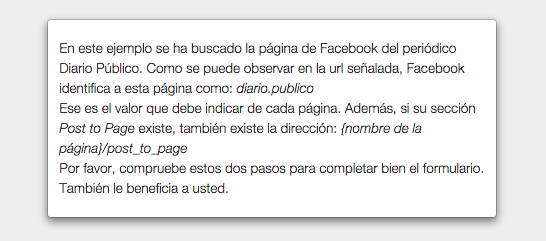
\includegraphics[width=3in]{figuras/help.png}
\caption{Captura de pantalla del diálogo de ayuda del paso 2} \label{fig:hel}
\end{figure}
Este paso es necesario ya que en Facebook existen muchas páginas con nombres similares pero de contenido totalmente opuesto, de esta forma, el usuario se asegura de que la página que se va a analizar es la correcta. 
\item Paso 3/4 \\
\begin{figure}[H]
\centering
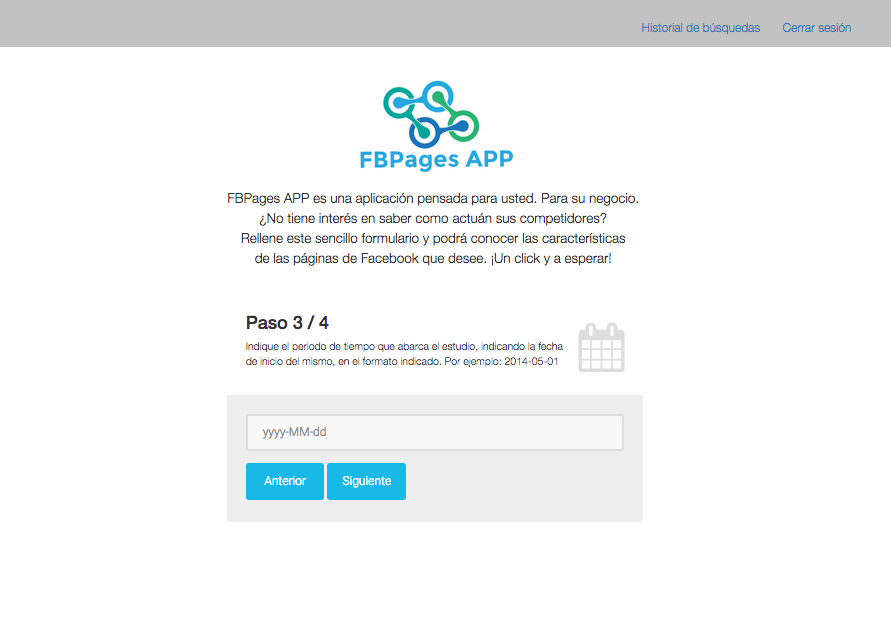
\includegraphics[width=5in]{figuras/paso3.png}
\caption{Captura de pantalla del Paso 3} \label{fig:paso3}
\end{figure}
En este paso el usuario debe indicar la fecha de inicio del estudio. Con este dato, la petición realizada a la API de Facebook se realizará desde la fecha de inicio hasta la fecha actual. Con este dato, el usuario puede decidir si quiere realizar un análisis de las últimas semanas, meses o años. \\
\\
\item Paso 4/4 \\
\begin{figure}[H]
\centering
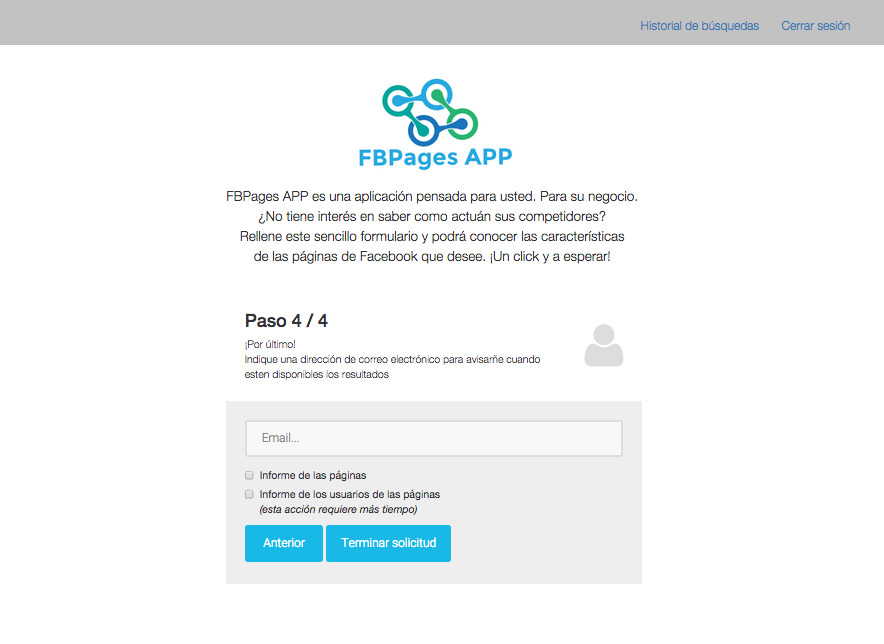
\includegraphics[width=5in]{figuras/paso4.png}
\caption{Captura de pantalla del Paso 4} \label{fig:paso4}
\end{figure}
Por último, el usuario debe indicar la dirección de correo donde quiere que se le avise cuando el estudio haya terminado de recopilar los datos. 
\end{itemize}

Una vez completado el formulario, el controlador "PageController.java" se encarga de almacenar esta búsqueda en la base de datos en la colección "pages", además de incluir los datos de la búsqueda introducidos por el usuario, también se añade al documento de la base de datos el "ID" del usuario, de forma que se pueda relacionar cada búsqueda con su usuario correspondiente. 

Acto seguido, el controlador se encarga de llamar a la siguiente acción. De cara al usuario, aparece una pantalla en la que se le indica que se están recogiendo los datos y que una vez haya acabado este proceso se le enviará un correo electrónico para notificárselo, tal y como se muestra en la siguiente figura (\ref{fig:working}).
\begin{figure}[H]
\centering
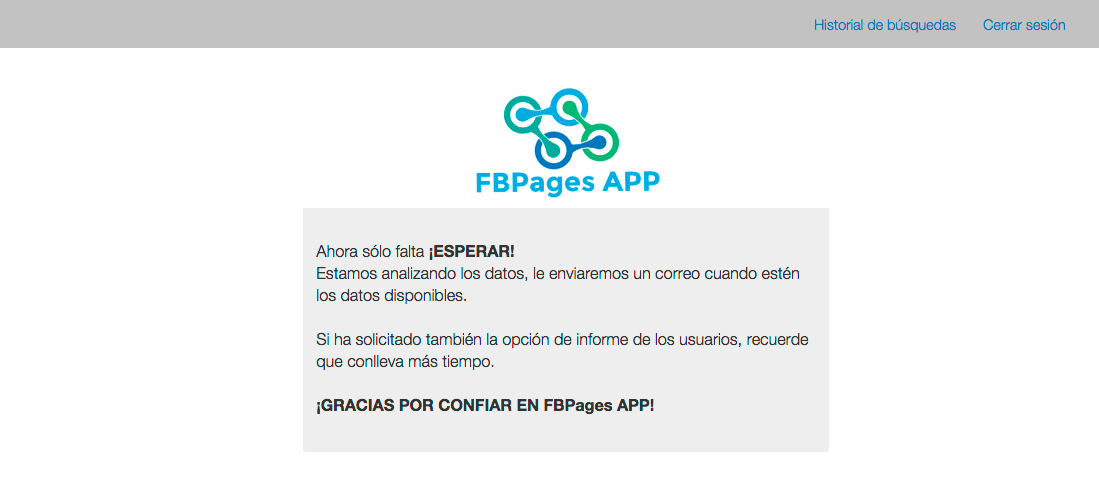
\includegraphics[width=4in]{figuras/working.png}
\caption{Captura de pantalla de la página de espera} \label{fig:working}
\end{figure}
No es tan sencillo como el usuario puede apreciar. Del controlador "PageController.java" se llama al controlador "WorkingController.java". Este controlador lo primero que hace es redirigir la página web a la vista "waiting.jsp" mostrada en la anterior figura. Esta vista está manejada por el controlador "WaitingController.java" que sólo se encarga de mostrar dicha vista. 

Por otro lado, el controlador  "WorkingController.java" inicia una tarea asíncrona. Una tarea asíncrona es aquella que es realiza en segundo plano para no alterar el flujo de la aplicación. 
Para manejar tareas asíncronas en una aplicación web en Spring MVC, se ha creado un \textit{Servlet} asíncrono. 
Un \textit{Servlet} es una clase de lenguaje de programación Java, utilizada para ampliar las capacidades de un servidor. Son utilizados para manejar las páginas web de forma dinámica a partir de los parámetros de la petición que envíe el navegador. Un \textit{Servlet} asíncrono tiene además la función de manejar hilos de tareas que requieren un largo tiempo de espera, de esta forma el navegador no está cargando hasta que se finalice la tarea. 

En la siguiente figura \ref{fig:sa} se muestra el esquema de funcionamiento de un \textit{Servlet} asíncrono. 
\begin{figure}[H]
\centering
\includegraphics[width=4in]{figuras/Servletasincrono.png}
\caption{Ejemplo de funcionamiento de un \textit{Servlet} asíncrono} \label{fig:sa}
\end{figure} 

La tarea asíncrona que maneja este controlador es la conexión con la API de Facebook para sacar los datos de las páginas solicitadas, esta función se explica en detalle más adelante en la sección (\ref{sec:4.2.2}). 

Una vez completada esta tarea, el controlador realiza dos pasos. Por un lado, envía un correo electrónico al usuario para notificarle que el estudio de las páginas de Facebook ha terminado, enviando el enlace donde puede acceder para ver los resultados. Por otro lado, envía un correo al administrador de la aplicación, en este caso la propia autora del trabajo fin de grado, para indicar que se ha solicitado el estudio de usuarios de las páginas, esta parte del proyecto se ha definido así porque el \textit{crawler} requiere ciertos servicios que deben estar correctamente activados antes de lanzarlo automáticamente, el funcionamiento de esta parte se explica más adelante en el sección (\ref{sec:4.2.3}).

\subsection{Historial}
\begin{figure}[H]
\centering
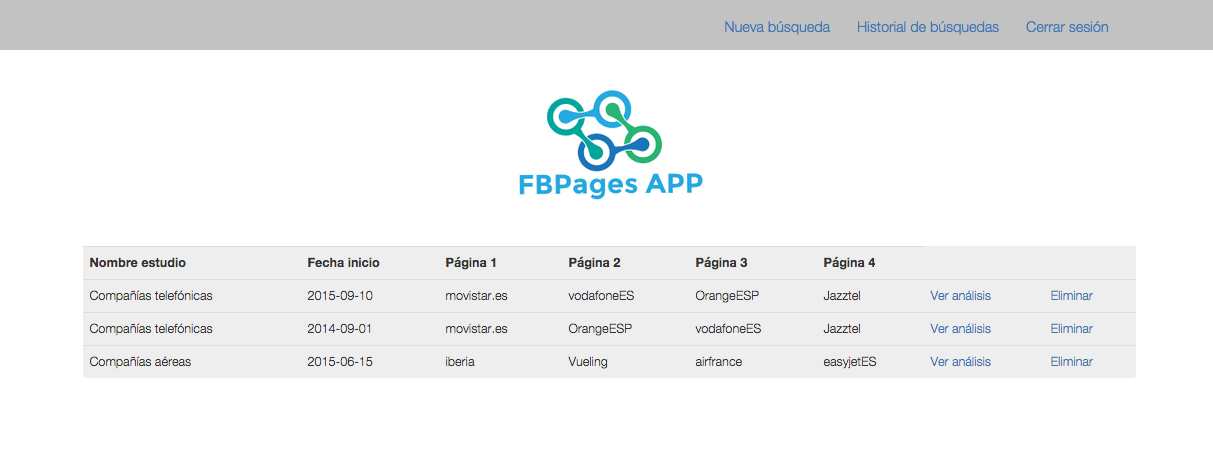
\includegraphics[width=5in]{figuras/historial.png}
\caption{Captura de pantalla de la página Historial} \label{fig:historial}
\end{figure}
Otra de las funciones a las que tiene acceso el usuario es a ver todos los estudios que ha solicitado en la aplicación. Esta vista muestra una tabla con todos los datos relacionados con el usuario. Desde esta tabla el usuario tiene dos acciones: "Ver el análisis" del estudio que elija o "Eliminar" esa búsqueda. 

Internamente el controlador "HistoryController.java" solicita a la base de datos "pages" que le devuelva todos los objetos que contienen el "ID" de usuario que corresponden con el que ha iniciado sesión en la aplicación, y devuelve la lista de páginas a la vista que se renderiza en la tabla que se observa en la figura (\ref{fig:historial}).

Además, si el usuario pulsa en la opción "Ver análisis", el controlador redirecciona la página a la vista "graphs.jsp" que es la encargada de mostrar los gráficos diseñados para la búsqueda seleccionada. 

Si por el contrario el usuario selecciona la opción "Eliminar", el controlador mediante una operación sencilla del CRUD definido para las páginas, eliminará esa entrada de la base de datos.
 
\subsection{Resultados} \label{sec:4.1.5}
Por último, la vista que muestra los resultados de un estudio concreto. Los usuarios pueden acceder a esta vista pulsando en el link que se les envía por correo electrónico o desde el historial, pulsando en la opción "Ver análisis". Pulsando en dicha opción, el usuario vería la siguiente pantalla que se muestra en la siguiente figura (\ref{fig:resultados})
\begin{figure}[H]
\centering
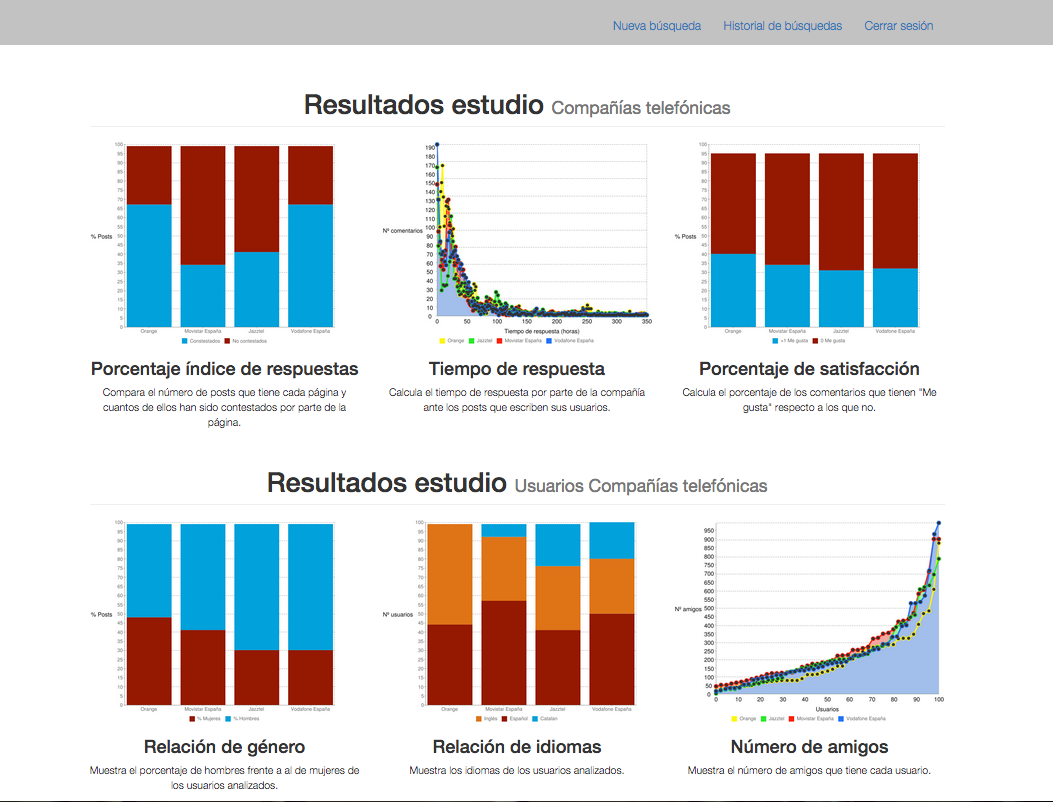
\includegraphics[width=5in]{figuras/ejemploCompleto.png}
\caption{Captura de pantalla del resultado del análisis} \label{fig:resultados}
\end{figure}

Esta vista se maneja por el controlador "ChartController.java". Se encarga de procesar los datos recogidos en la base de datos de MySQL con el nombre concreto de la búsqueda y los representa en gráficas mediante Google Chart. 

Google Chart es un herramienta para desarrolladores que permite la creacción de gráficas en forma de imágenes PNG para poder utilizarlas en las páginas web. Para utilizar esta herramienta se ha utilizado una librería de java "charts4j" \cite{charts} que permite integrar las funcionalidades de Google Chart en la aplicación. 

Se han definido las gráficas por defecto, lo único que cambian son los datos que las definen, que son cogidos de la base de datos. En el siguiente listado se muestran todas las gráficas que se han realizado y un ejemplo de cada una de ellas: 
\begin{enumerate}
\item \textbf{ESTUDIO BASADO EN LAS PÁGINAS DE FACEBOOK}
\begin{itemize}
\item \textbf{Porcentaje índice de respuesta}\\
\begin{figure}[H]
\centering
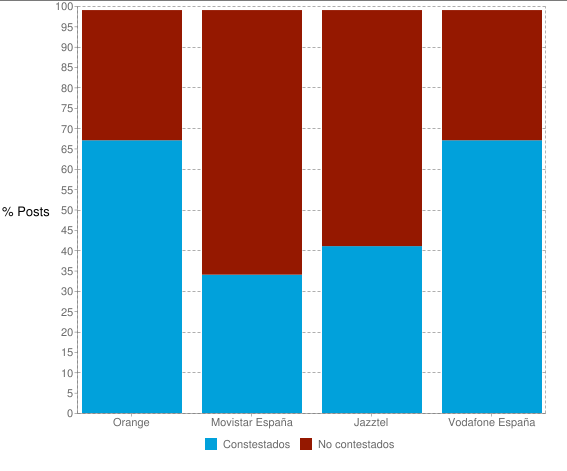
\includegraphics[width=2in]{figuras/contestados.png}
\caption{Gráfica porcentaje índice de respuesta} \label{fig:contestados}
\end{figure}
Esta gráfica presenta los resultados de los datos obtenidos, obteniendo el porcentaje del total de los comentarios que ha contestado la página bajo estudio frente a los que no.  

\item \textbf{Tiempo de respuesta}\\
\begin{figure}[H]
\centering
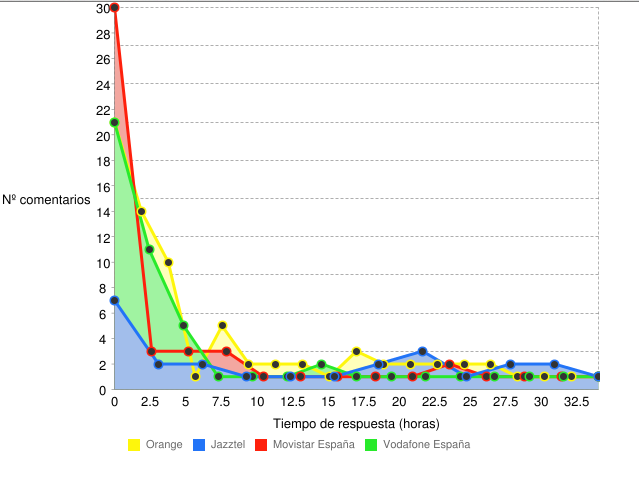
\includegraphics[width=2in]{figuras/tiempo.png}
\caption{Gráfica tiempo de respuesta} \label{fig:tiempo}
\end{figure}
Esta gráfica muestra el tiempo de respuesta por parte de la página a los comentarios que escriben los usuarios. Este tiempo está calculado en horas.
\item \textbf{Porcentaje de satisfacción}\\
\begin{figure}[H]
\centering
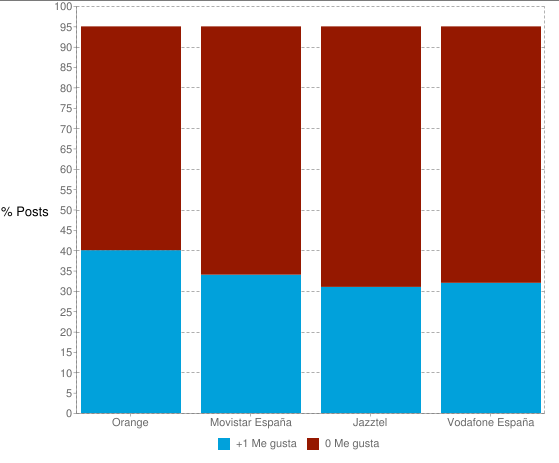
\includegraphics[width=2in]{figuras/satisfaccion.png}
\caption{Gráfica porcentaje de satisfacción} \label{fig:satisfaccion}
\end{figure}
Este gráfico representa el porcentaje de comentarios que han obtenido algún "Me gusta" (\textit{Likes}, comúnmente conocido) frente a los que no. 
\end{itemize}
\item \textbf{ESTUDIO BASADO EN LOS USUARIO DE LAS PÁGINAS DE FACEBOOK}
\begin{itemize}
\item \textbf{Relación de género}\\
\begin{figure}[H]
\centering
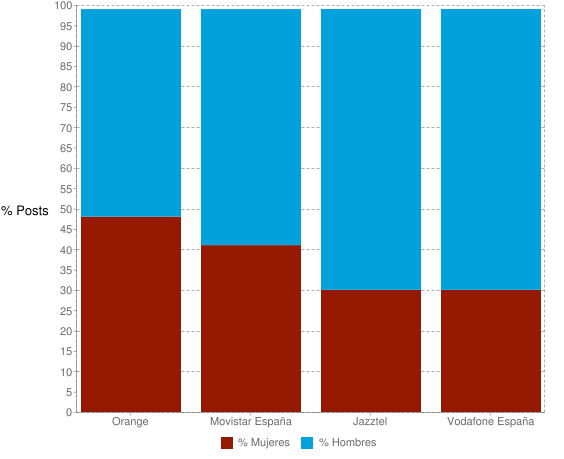
\includegraphics[width=2in]{figuras/genero.png}
\caption{Gráfica relación de genero} \label{fig:genero}
\end{figure}
Esta gráfica muestra el porcentaje de hombres y mujeres dentro de los usuarios analizados de cada página.  
\item \textbf{Relación de idiomas}\\
\begin{figure}[H]
\centering
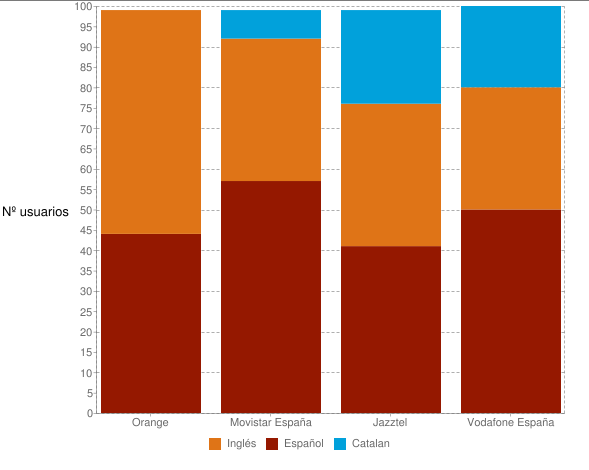
\includegraphics[width=2in]{figuras/idioma.png}
\caption{Gráfica relación de genero} \label{fig:idioma}
\end{figure}
Esta gráfica representa el porcentaje de usuarios de habla ingles, española o catalana. Aunque no es un dato muy fiable, dado que muchos usuarios dominarán más del idioma materno, por norma general, aquellos usuarios que especifican un idioma, indican su propia lengua materna.
\item \textbf{Número de amigos}\\
\begin{figure}[H]
\centering
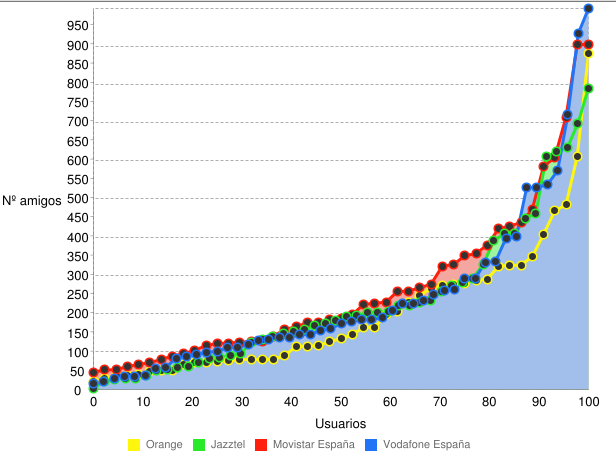
\includegraphics[width=2in]{figuras/amigos.png}
\caption{Gráfica número de amigos} \label{fig:amigos}
\end{figure}
En esta gráfica se muestra el número de amigos que tiene cada uno de los usuarios analizados. El fin de esta gráfica es considerar si son cuentas activas o no, ya que si el porcentaje de usuarios con cero amigos es muy elevado, podría indicar que son usuarios falsos.
\end{itemize}
\end{enumerate}

\section{Backend}
En el lado del servidor tenemos una estructura más compleja, que se va a explicar dividiéndolo en cada una de las herramientas utilizadas o creadas para el correcto funcionamiento de la aplicación.
Primeramente, se va a mostrar el diagrama completo del backend, tal y como se muestra en la figura (\ref{fig:backend}). 
\begin{figure}[H]
\centering
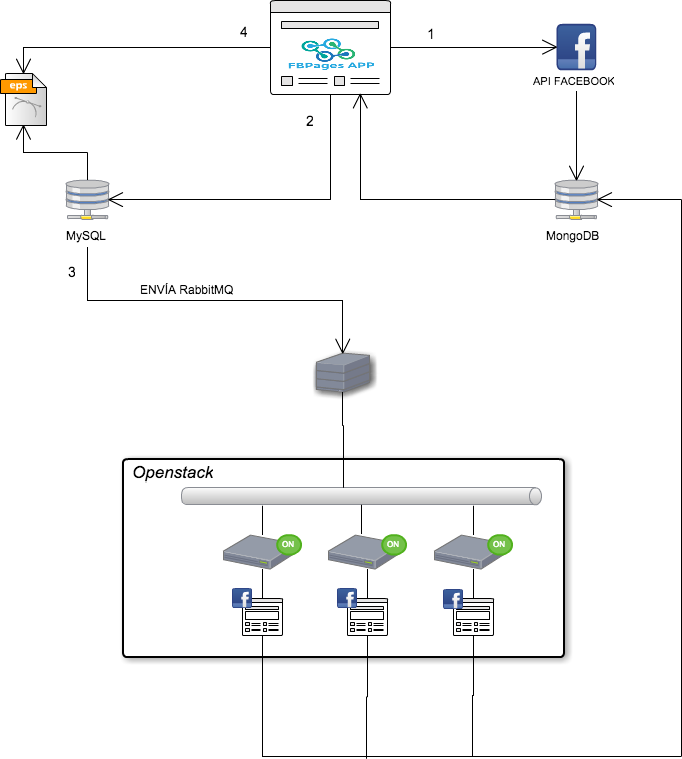
\includegraphics[width=4in]{figuras/backend.png}
\caption{Esquema funcionamiento backend} \label{fig:backend}
\end{figure}

Como se puede observar en la anterior figura, hay varios pasos implementados, que tienen que seguir el orden indicado para poder obtener todos los datos requeridos.

\subsection{API Facebook Developers} \label{sec:4.2.2}
El primer paso indicado es la API de Facebook. El usuario en la aplicación indicará los datos necesarios para realizar la consulta a la API, una vez obtenidos esos datos por parte del usuario, se lanza un script, de manera asíncrona, tal y como se ha explicado en la sección (\ref{sec:4.1.3}). En este punto se va a explicar más en detalle como funciona este programa.

La API de Facebook es la principal forma de obtener los datos dentro y fuera del gráfico social de Facebook. Es una API basada en HTTP que se ha utilizado para consultar datos. A continuación se muestra un ejemplo de una petición a la API de Facebook, mediante su herramienta \textit{Graph API}. Esta herramienta permite ver los resultados de la consulta que se desea hacer. 
\begin{figure}[H]
\centering
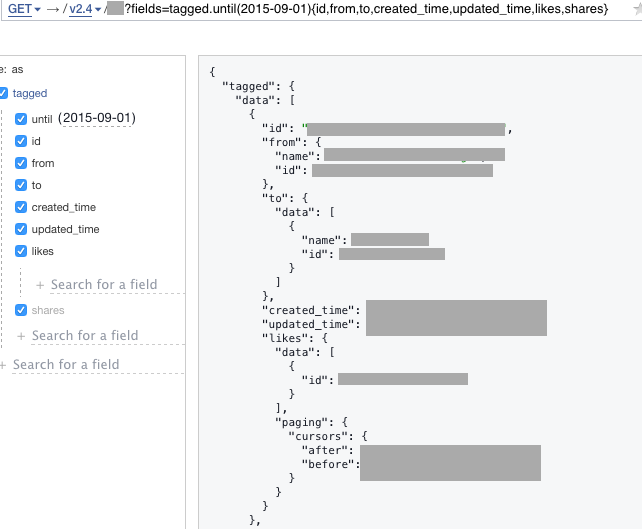
\includegraphics[width=4in]{figuras/ejemploAPI.png}
\caption{Esquema petición API Facebook} \label{fig:ejemploAPI}
\end{figure}

Para poder obtener los datos de las páginas de Facebook indicadas por el usuario de forma automática, se ha creado un programa que realiza las peticiones a la API de Facebook con los parámetros necesarios, en nuestro caso de la sección \textit{tagged}, que se corresponde con los posts de los usuarios en las páginas. 

La API de Facebook devuelve en formato JSON los resultados, este fichero es almacenado directamente en la base de datos de MongoDB, para su posterior procesado.

Esta acción se repite para cada una de las páginas indicadas por el usuario, hasta completar la obtención de datos necesaria. 

El segundo paso consiste en leer los datos obtenidos y almacenados en MongoDB, coger sólo aquellos datos de interés para este trabajo fin de grado y ordenarlos en una tabla en MySQL. De esta forma, es más fácil acceder a ellos y representarlos.

\subsection{Distribución: RabbitMQ}
Una vez guardados los datos en MySQL, si el usuario ha seleccionado la opción de "Informe de los usuarios de las páginas", el siguiente paso es lanzar el \textit{crawler} para recoger los datos de los usuarios. 

Antes de explicar el funcionamiento del \textit{crawler}, se va a explicar la arquitectura desplegada mediante RabbitMQ para la correcta distribución del \textit{crawler}. Como se ha explicado en el Estado del Arte, RabbitMQ es un sistema de intercambio de mensajes. La utilización en este trabajo fin de grado se basa en el envío de mensajes a cuatro máquinas virtuales en las que se ejecutará el \textit{crawler}. 

El sistema es muy sencillo, se configuran las cuatro máquinas virtuales con el entorno necesario para ejecutar el \textit{crawler}. Una vez hecho esto, se lanza el script de RabbitMQ que tiene la función de recibir. Cada VM recibe mensajes de una cola de mensajes distinta, por lo que el emisor es el encargado de decidir que envía a cada VM, o lo que es lo mismo a cada cola. 

Por otro lado, desde la aplicación se maneja el script encargado de enviar los mensajes. Este script manda un mensaje a cada una de las colas de mensajes activas indicando el número de usuarios a analizar y el nombre de la página de donde han sido extraídos. Una vez enviado el mensaje, se queda esperando para recibir la confirmación de que el trabajo ha finalizado. De esta forma, se distribuye el \textit{crawler} en cada máquina virtual de forma automática, sin necesidad de ir a cada una de las VMs para lanzar el \textit{crawler}.

\subsection{Crawler de Facebook: Selenium WebDriver} \label{sec:4.2.3}

El \textit{crawler} es un script escrito en Java, que tiene como función principal recoger los datos de un usuario de Facebook. Se basa en reproducir los pasos que haría un humano si mirase el perfil de un usuario en Facebook. 

Este \textit{crawler} funciona lanzando una instancia del navegador Firefox,  indicando la url de Facebook. Como toda persona que pertenece a esta comunidad, lo primero que debe hacer es iniciar sesión con una cuenta existente, y una vez dentro, procede a visitar los perfiles de cada uno de los usuarios que se le han indicado. El número de usuarios estipulado para este proyecto han sido 100, número suficiente para poder perfilar los patrones de los usuarios más comunes de una página web.

La instancia que lanza en navegador recibe el nombre de WebDriver, permite configurar y ejecutar los comandos necesarios para parsear la web y coger los datos deseados. 

Los datos recogidos de los usuarios en Facebook, son almacenados de igual forma que los de la API de Facebook, se crea un objeto JSON con todos los campos obtenidos del perfil y se almacena directamente en MongoDB. Se ha definido de esta forma por si en un futuro cambian los campos del perfil de un usuario de Facebook, añadiendo o eliminando algún campo, solo habría que modificar el fichero JSON que se va a introducir en la base de datos, sin necesidad de modificar nada más. 

\subsection{Análisis gráfico: Google Chart}

Por último, el cuarto paso consiste en analizar todos los datos obtenidos tanto de la API de Facebook como del \textit{crawler} para representarlos gráficamente y que el usuario pueda verlo en la interfaz de la aplicación. 

Para representar los datos se ha utilizado la herramienta de Google Chart, que facilita la integración de las gráficas con una aplicación web. Esta herramienta es utilizada en este proyecto mediante una librería de java, ya comentada anteriormente en la sección (\ref{sec:4.1.5}). Se define el tipo de gráfica que se quiere representar, y se le pasa como parámetro los datos ya procesados, Google Chart se encarga de dibujarlos en las gráficas.

Hay dos grandes bloques de datos que se han almacenado en la base de datos para ser procesados, los de los usuarios y los de las páginas de Facebook. 

Por un lado, los datos relacionados con los usuarios, extraídos mediante el \textit{crawler}. De estos datos se obtiene la información de los usuarios en relación a su género, número de amigos e idiomas hablados y se calcula el porcentaje de cada una de las variables para cada página. Una vez calculados los porcentajes, se representan en una tabla conjunta para ver la diferencia de porcentaje entre cada página. 

Por parte de los datos obtenidos de la API de Facebook se han tenido en cuenta la fecha de creación de un mensaje y la fecha de actualización del mismo, si no existe la fecha de actualización significa que la página de Facebook no ha contestado al comentario, y si por el contrario existe, se calcula la diferencia de tiempo, pudiendo así obtener el tiempo de respuesta de la página de Facebook ante un comentario. Con estos dos datos, se obtienen las gráficas del porcentaje de respuesta y del tiempo de respuesta explicadas en la sección (\ref{sec:4.1.5}). También se extrae el dato de número de "Me gusta" que tiene cada comentario para calcular el porcentaje de satisfacción de los usuarios ante las publicaciones recogidas. 
